\section{Appendix}

% ------------- Appendix Figures -------------
% Figures to be placed in the appendix

\begin{figure}[H]
	\centering
	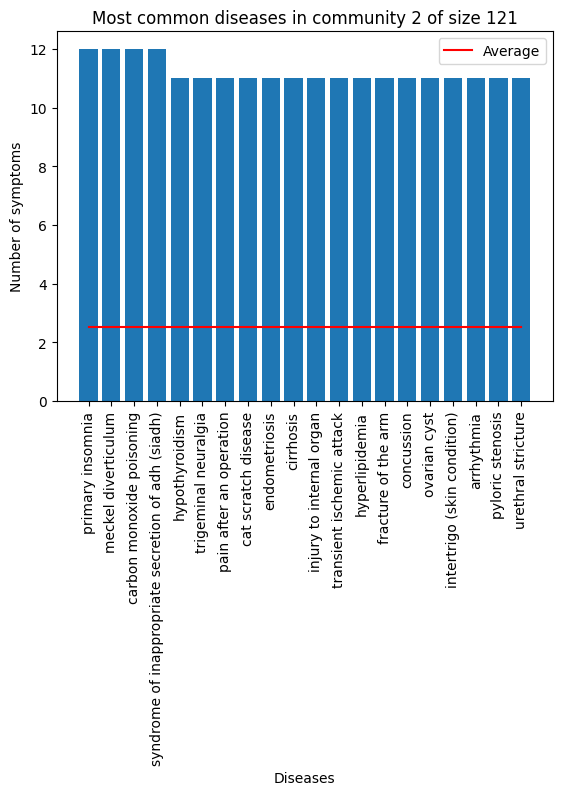
\includegraphics[width=\columnwidth]{com2_symptoms.png}
	\caption{Community 2 of symptoms}\label{fig:com2_symptoms}
\end{figure}
\noindent
\begin{figure}[H]
	\centering
	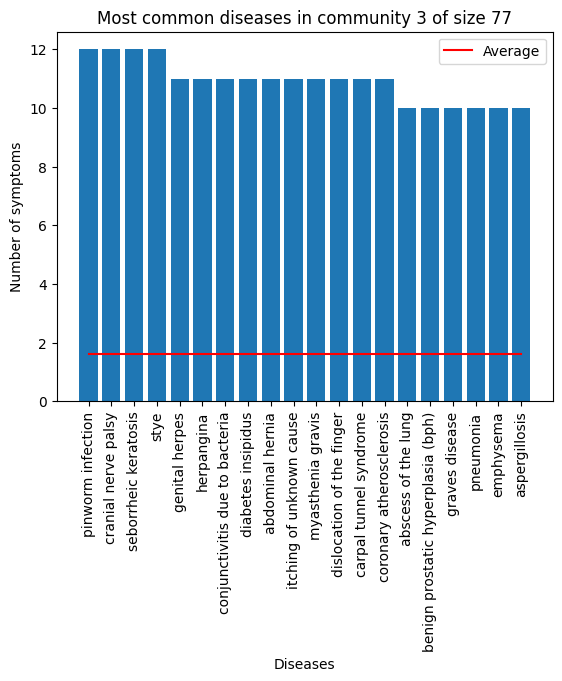
\includegraphics[width=\columnwidth]{com3_symptoms.png}
	\caption{Community 3 of symptoms}\label{fig:com3_symptoms}
\end{figure}
\noindent


\begin{figure}[H]
	\centering
	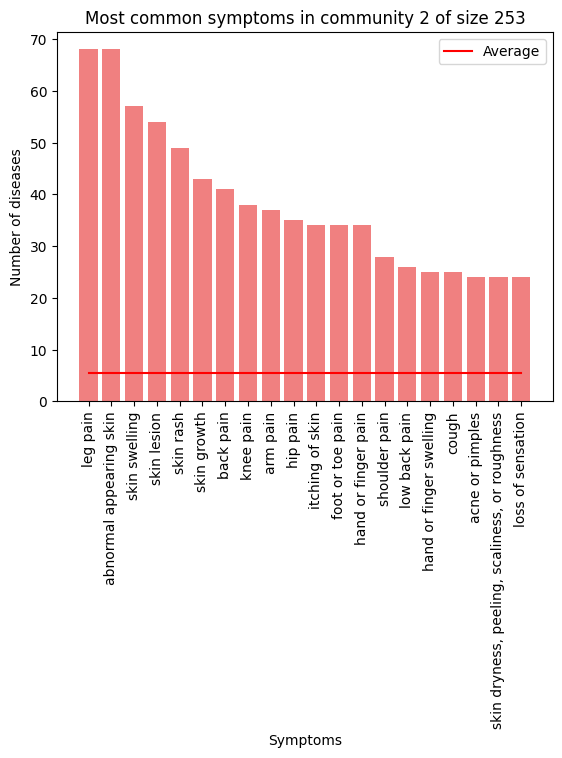
\includegraphics[width=\columnwidth]{com2_diseases.png}
	\caption{Community 2 of diseases}\label{fig:com2_diseases}
\end{figure}
\noindent
\begin{figure}[H]
	\centering
	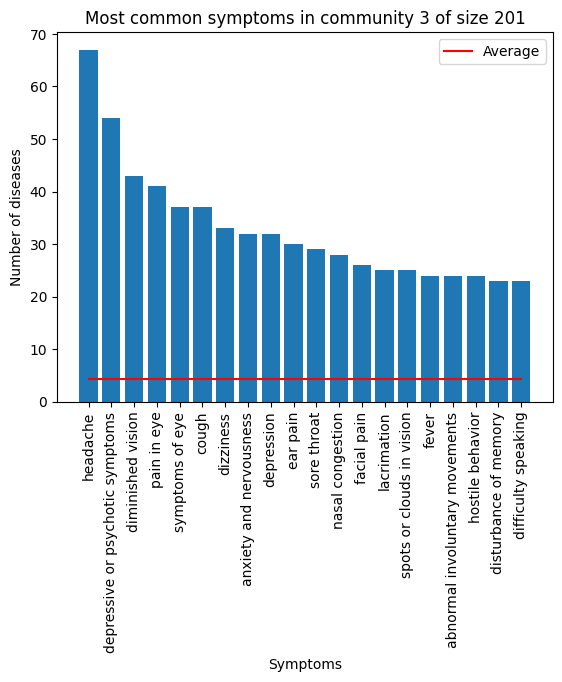
\includegraphics[width=\columnwidth]{com3_diseases.png}
	\caption{Community 3 of diseases}\label{fig:com3_diseases}
\end{figure}
\noindent


\begin{figure}[H]
	\centering
	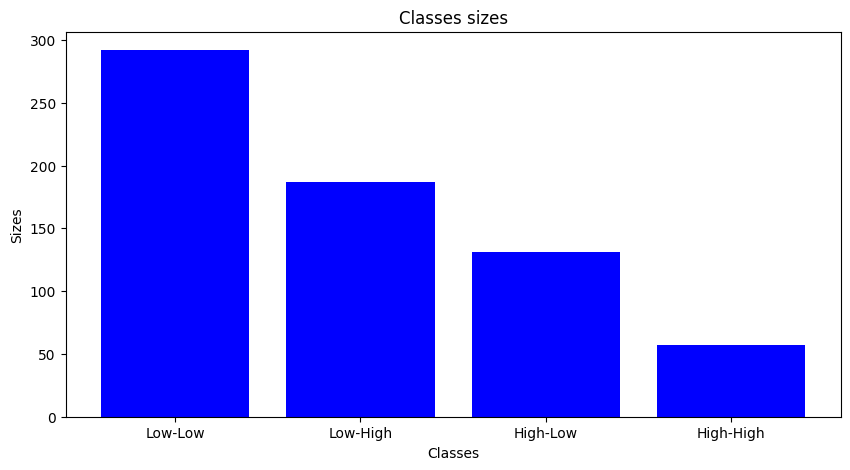
\includegraphics[width=\columnwidth]{diseases_classes.png}
	\caption{Diseases divided into the four classes}\label{fig:diseases_classes}
\end{figure}

\begin{figure*}[!t]
	\centering
	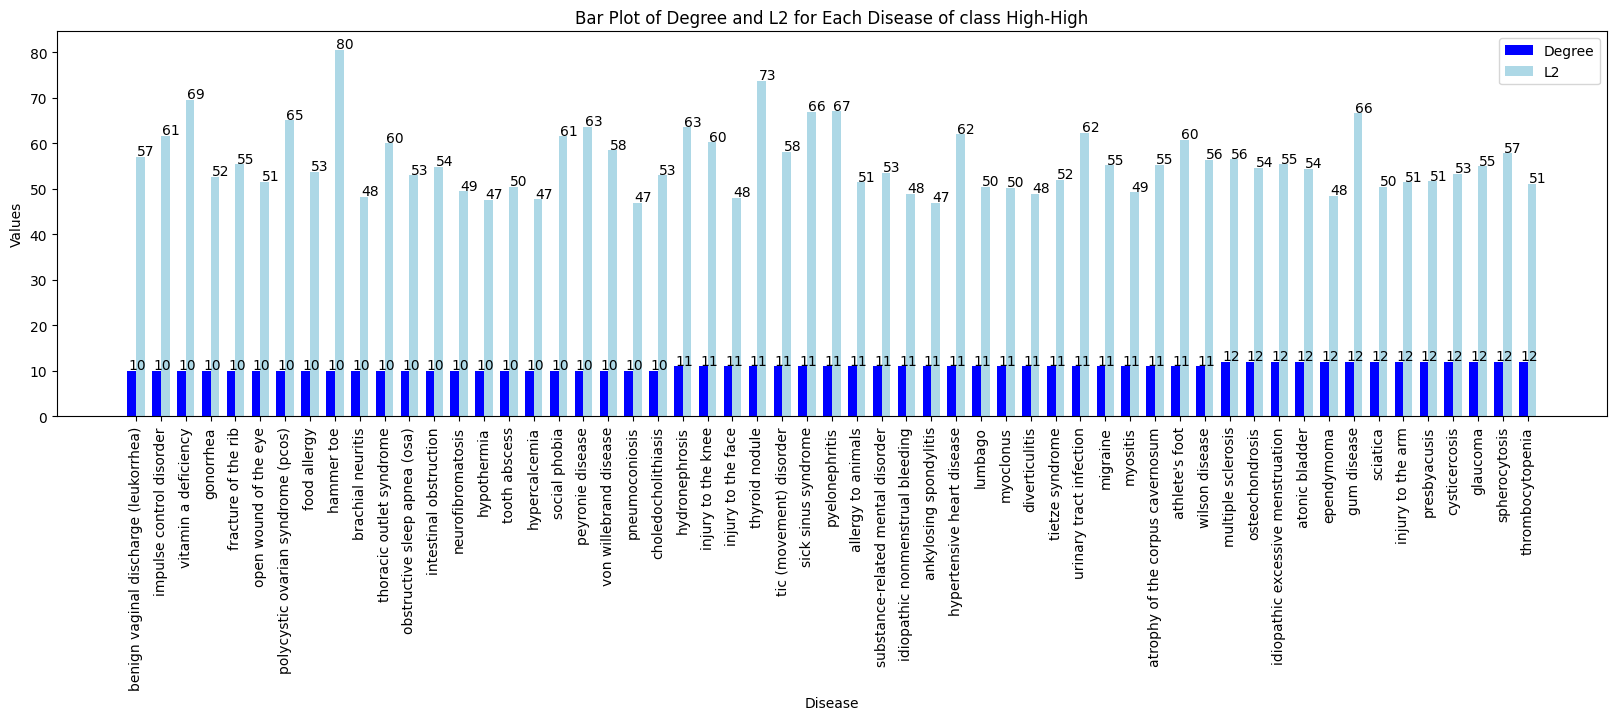
\includegraphics[width=\textwidth]{hig_l1_hig_l2_class.png}
	\caption{Composition of the high-L1-high-L2 class for diseases}\label{fig:high_l1_high_l2_class}
\end{figure*}